%HW03.tex
%
% Third Homework for Graduate Algebra
% Frank Sottile
%%%%%%%%%%%%%%%%%%%%%%%%%%%%%%%%%%%%%%%%%%%%%%%%%%%%%%%%%%%%%%%%%%%%%%%
\documentclass[12pt]{article}
\usepackage{multicol,amsfonts, amssymb,  mathtools,amsmath}
\usepackage{colordvi,graphicx}
\headheight=8pt
%
\topmargin=-85pt
\textheight=720pt   \textwidth=560pt
\oddsidemargin=-60pt \evensidemargin=-60pt

\pagestyle{empty}

%%%%%%%%%%%%%%%%%%%%%%%%%%%%%%%%%%%%%%%%%%%%
\newcommand{\CC}{{\mathbb C}}
\newcommand{\KK}{{\mathbb K}}
\newcommand{\NN}{{\mathbb N}}
\newcommand{\QQ}{{\mathbb Q}}
\newcommand{\RR}{{\mathbb R}}
\newcommand{\TT}{{\mathbb T}}
\newcommand{\ZZ}{{\mathbb Z}}

\newcommand{\calA}{{\mathcal A}}
\newcommand{\be}{{\bf e}}
\newcommand{\bfi}{{\bf i}}
\newcommand{\bfj}{{\bf j}}

\newcommand{\Aut}{\mbox{Aut}}
\newcommand{\Hom}{\mbox{Hom}}
\newcommand{\spec}{\mbox{spec}}
\newcommand{\cone}{\mbox{cone}}

\newcommand{\vect}[2]{(\begin{smallmatrix}#1\\#2\end{smallmatrix})}
\newcommand{\msp}{\hspace{8pt}}
%\newcommand{\Square}{\raisebox{-2pt}{\includegraphics{images/Square.eps}}}
\newcommand{\Square}{\raisebox{-2pt}{\Large$\square$}}

\def\Color#1#2{\special{color push cmyk #1}#2\special{color pop}}
%\def\Indigo#1{\Color{.42 1. 0. .49}{#1}}
\def\Indigo#1{\Color{1. .95 .05 .4}{#1}}
\def\MyViolet#1{\Color{.6 1. 0. .15}{#1}}
\def\TAMU#1{\Color{.15 1. .39 .69}{#1}}

\newcommand{\barsl}{\noindent\begin{minipage}[t]{590pt}
\Indigo{\rule{590pt}{1.2pt}}\vspace{-5.7mm}\\
\MyViolet{\rule{590pt}{1.2pt}}\vspace{-5.7mm}\\
\Blue{\rule{590pt}{1.2pt}}\vspace{-5.7mm}\\
\Green{\rule{590pt}{1.2pt}}\vspace{-5.7mm}\\
\Yellow{\rule{590pt}{1.2pt}}\vspace{-5.7mm}\\
\Orange{\rule{590pt}{1.2pt}}\vspace{-5.7mm}\\
\Red{\rule{590pt}{1.2pt}}\bigskip
\end{minipage}}


\newcommand{\barsn}{\noindent\begin{minipage}[t]{590pt}
\Indigo{\rule{590pt}{1.1pt}}\vspace{-4.5mm}\\
\MyViolet{\rule{590pt}{1.1pt}}\vspace{-4.5mm}\\
\Blue{\rule{590pt}{1.1pt}}\vspace{-4.5mm}\\
\Green{\rule{590pt}{1.1pt}}\vspace{-4.5mm}\\
\Yellow{\rule{590pt}{1.1pt}}\vspace{-4.5mm}\\
\Orange{\rule{590pt}{1.1pt}}\vspace{-4.5mm}\\
\Red{\rule{590pt}{1.1pt}}\bigskip
\end{minipage}}

\def\demph#1{\TAMU{{\sl #1}}}
\def\defcolor#1{\TAMU{#1}}

\begin{document}
\LARGE 
\noindent
Algebra \ \ Autumn 2025\vspace{1pt}\\
Frank Sottile\vspace{2pt}\\
\Large 4 September 2025 \hfill
\sf
 Third Homework\makebox[20pt][l]{\ }
\normalsize\vspace{10pt}

\noindent
Write your answers neatly, in complete sentences.  
I highly recommend recopying your work before handing it in.
Correct and crisp proofs are greatly appreciated; oftentimes your work can be shortened and made clearer.

You will note that some problems were partially done in class.
This is an opportunity to polish your skills at writing mathematics in a clear and organized manner.

\barsn

\noindent\Maroon{{\sf Hand in {\bf to Frank, on a separeate sheet} at the start of class, Thursday 11 September:}} 

\begin{enumerate}
\setcounter{enumi}{12}

%%%%%%%%%%%%%%%%%%%%%%%%%%%%%%%%%%%%%%%%%%%%%%%%%%%%%%%%%%%%%%%%%%%%%%%%%%%%%%%%%%%%%%%%%%%%%%%%%%%%
\item 
   Let $H,K$ be subgroups of a group $G$.
      Show that any left coset of $H\cap K$ is the intersection of a left coset of $H$ with a
      left coset of $K$.
      Use this to prove Poincar\'e's Theorem that if $H$ and $K$ have finite index, then so
      does $H\cap K$.
%%%%%%%%%%%%%%%%%%%%%%%%%%%%%%%%%%%%%%%%%%%%%%%%%%%%%%%%%%%%%%%%%%%%%%%%%%%%%%%%%%%%%%%%%%%%%%%%%%%%  


\end{enumerate}
%%%%%%%%%%%%%%%%%%%%%%%%%%%%%%%%%%%%%%%%%%%%%%%%%%%%%%%%%%%%%%%%%%%%%%%%%%%%%%%%%%%%%%%%%%%%%%%%%%%%


\barsn

\noindent\Maroon{{\sf Hand in at the start of class, Thursday 11 September:}} 

\begin{enumerate}
\setcounter{enumi}{13}

%%%%%%%%%%%%%%%%%%%%%%%%%%%%%%%%%%%%%%%%%%%%%%%%%%%%%%%%%%%%%%%%%%%%%%%%%%%%%%%%%%%%%%%%%%%%%%%%%%%%
\item  Let $G$ be a group.
  For $g\in G$, show that conjugation by $g$, $G\ni a\mapsto gag^{-1}=\vcentcolon {^ga}$ is an automorphism of $G$.
  This is called an \demph{inner automorphism}.

  Show that the set of inner automorphisms of $G$ forms a normal subgroup of $\Aut(G)$, the group of all automorphisms of $G$.
%%%%%%%%%%%%%%%%%%%%%%%%%%%%%%%%%%%%%%%%%%%%%%%%%%%%%%%%%%%%%%%%%%%%%%%%%%%%%%%%%%%%%%%%%%%%%%%%%%%%


%%%%%%%%%%%%%%%%%%%%%%%%%%%%%%%%%%%%%%%%%%%%%%%%%%%%%%%%%%%%%%%%%%%%%%%%%%%%%%%%%%%%%%%%%%%%%%%%%%%%
\item 
    Suppose that $\varphi\colon G\to H$ is a group homomorphism.
    If $\varphi$ is a bijection, then the inverse function $\varphi^{-1}\colon H\to G$ is also a homomorphism.  
    (Do this by checking that it preserves the identity, sends products to products, and sends inverses to inverses.)
%%%%%%%%%%%%%%%%%%%%%%%%%%%%%%%%%%%%%%%%%%%%%%%%%%%%%%%%%%%%%%%%%%%%%%%%%%%%%%%%%%%%%%%%%%%%%%%%%%%%  

%%%%%%%%%%%%%%%%%%%%%%%%%%%%%%%%%%%%%%%%%%%%%%%%%%%%%%%%%%%%%%%%%%%%%%%%%%%%%%%%%%%%%%%%%%%%%%%%%%%%
\item 
   Let $S\subset G$ be a subset of a group $G$ and define the relation 
\defcolor{$\sim$} by  $a\sim b$ if and only if $ab^{-1}\in S$.
Show that $\sim$ is an equivalence relation if and only if $S$ is a subgroup of $G$.
%%%%%%%%%%%%%%%%%%%%%%%%%%%%%%%%%%%%%%%%%%%%%%%%%%%%%%%%%%%%%%%%%%%%%%%%%%%%%%%%%%%%%%%%%%%%%%%%%%%%  
    
%%%%%%%%%%%%%%%%%%%%%%%%%%%%%%%%%%%%%%%%%%%%%%%%%%%%%%%%%%%%%%%%%%%%%%%%%%%%%%%%%%%%%%%%%%%%%%%%%%%%
\item  Let $H$ be a subgroup of a group $G$.
  Define the \demph{normalizer} of $H$ in $G$ to be
  \[
     \defcolor{N_G(H)}\ \vcentcolon=\ \{g\in G\mid gHg^{-1} = H\}\,.
  \]
  \begin{enumerate}
    \item Prove that $N_G(H)$ is a subgroup of $G$ that contains $H$.
    \item Let $K$ be a subgroup of $G$ that contains $H$.  
          Prove that if $H$ is normal in $K$, then $K\subset N_G(H)$.
    \item Let $K$ be a subgroup of $N_G(H)$.  
          Prove that $KH$ is a group and $H$ is normal in $KH$.
          Recall from class that $KH\vcentcolon=\{kh\mid k\in K,\ h\in H\}$.
   \end{enumerate}
%%%%%%%%%%%%%%%%%%%%%%%%%%%%%%%%%%%%%%%%%%%%%%%%%%%%%%%%%%%%%%%%%%%%%%%%%%%%%%%%%%%%%%%%%%%%%%%%%%%%



%%%%%%%%%%%%%%%%%%%%%%%%%%%%%%%%%%%%%%%%%%%%%%%%%%%%%%%%%%%%%%%%%%%%%%%%%%%%%%%%%%%%%%%%%%%%%%%%%%%%
\item
      Let $p$ be the smallest prime number dividing the order $|G|$ of a finite group $G$ and
  suppose that $G$ has a subgroup $H$ of index $p$, $[G:H]=p$.
  Prove that $H$ is normal in $G$.
%%%%%%%%%%%%%%%%%%%%%%%%%%%%%%%%%%%%%%%%%%%%%%%%%%%%%%%%%%%%%%%%%%%%%%%%%%%%%%%%%%%%%%%%%%%%%%%%%%%%  

%%%%%%%%%%%%%%%%%%%%%%%%%%%%%%%%%%%%%%%%%%%%%%%%%%%%%%%%%%%%%%%%%%%%%%%%%%%%%%%%%%%%%%%%%%%%%%%%%%%%
\item  Prove that the absolute value map $\lvert \ \rvert \colon \CC^\times \to \RR^\times$ that sends a nonzero complex
  number to its absolute value is a group homomorphism, and determine its image and kernel.
%%%%%%%%%%%%%%%%%%%%%%%%%%%%%%%%%%%%%%%%%%%%%%%%%%%%%%%%%%%%%%%%%%%%%%%%%%%%%%%%%%%%%%%%%%%%%%%%%%%%

%%%%%%%%%%%%%%%%%%%%%%%%%%%%%%%%%%%%%%%%%%%%%%%%%%%%%%%%%%%%%%%%%%%%%%%%%%%%%%%%%%%%%%%%%%%%%%%%%%%%
\item  Suppose that $\varphi\colon G\twoheadrightarrow H$ is a surjective homomorphism of groups with kernel $N$.
  Show that $K\mapsto \varphi(K)$ and $L\mapsto \varphi^{-1}(L)$ are inverse bijections between,
  \begin{enumerate}
  \item $\{\mbox{subgroups $K$ of $G$ that contain $N$}\}$  and
              $\{\mbox{subgroups $L$ of $H$}\}$.

  \item $\{\mbox{normal subgroups $K$ of $G$ that contain $N$}\}$  and
              $\{\mbox{normal subgroups $L$ of $H$}\}$.

  \end{enumerate}
%%%%%%%%%%%%%%%%%%%%%%%%%%%%%%%%%%%%%%%%%%%%%%%%%%%%%%%%%%%%%%%%%%%%%%%%%%%%%%%%%%%%%%%%%%%%%%%%%%%%

\end{enumerate}
%%%%%%%%%%%%%%%%%%%%%%%%%%%%%%%%%%%%%%%%%%%%%%%%%%%%%%%%%%%%%%%%%%%%%%%%%%%%%%%%%%%%%%%%%%%%%%%%%%%%

\end{document}

%%%%%%%%%%%%%%%%%%%%%%%%%%%%%%%%%%%%%%%%%%%%%%%%%%%%%%%%%%%%%%%%%%%%%%%%%%%%%%%%%%%%%%%%%%%%%%%%%%%%
\item  
%%%%%%%%%%%%%%%%%%%%%%%%%%%%%%%%%%%%%%%%%%%%%%%%%%%%%%%%%%%%%%%%%%%%%%%%%%%%%%%%%%%%%%%%%%%%%%%%%%%%

